%%
% This is an Overleaf template for presentations
% using the TUM Corporate Desing https://www.tum.de/cd
%
% For further details on how to use the template, take a look at our
% GitLab repository and browse through our test documents
% https://gitlab.lrz.de/latex4ei/tum-templates.
%
% The tumbeamer class is based on the beamer class.
% If you need further customization please consult the beamer class guide
% https://ctan.org/pkg/beamer.
% Additional class options are passed down to the base class.
%
% If you encounter any bugs or undesired behaviour, please raise an issue
% in our GitLab repository
% https://gitlab.lrz.de/latex4ei/tum-templates/issues
% and provide a description and minimal working example of your problem.
%%


\documentclass[
  english,            % define the document language (english, german)
  aspectratio=169,    % define the aspect ratio (169, 43)
  % handout=2on1,       % create handout with multiple slides (2on1, 4on1)
  % partpage=false,     % insert page at beginning of parts (true, false)
  % sectionpage=true,   % insert page at beginning of sections (true, false)
]{tumbeamer}


% load additional packages
\usepackage{booktabs}
\usepackage{tikz}
\usetikzlibrary{positioning,arrows.meta,calc}
\usepackage{pgfplots}\pgfplotsset{compat=1.18}
\definecolor{accent}{HTML}{2A7DB0}
\definecolor{warm}{HTML}{D85A30}
\definecolor{teal}{HTML}{0F8A6B}
\definecolor{muted}{HTML}{888780}

% presentation metadata
\title{Minimising \texorpdfstring{$k$}{k} in Straight-Line Graph Drawings}
\subtitle{Intermediate Presentation -- Graph Drawing Contest k-planarity Solver}
\author{Amine \and Berkay \and Yi\u{g}it}

\institute{Chair for Efficient Algorithms (ALGO)\\Department of Computer Science\\Technical University of Munich}
\date[08/06/2026]{June 8\textsuperscript{th}, 2026}

\footline{\insertauthor~|~\insertshorttitle~|~\insertshortdate}


% macro to configure the style of the presentation
\TUMbeamersetup{
  title page = TUM tower,         % style of the title page
  part page = TUM toc,            % style of part pages
  section page = TUM toc,         % style of section pages
  content page = TUM more space,  % style of normal content pages
  tower scale = 1.0,              % scaling factor of TUM tower (if used)
  headline = TUM threeliner,      % which variation of headline to use
  footline = TUM default,         % which variation of footline to use
  % configure on which pages headlines and footlines should be printed
  headline on = {title page},
  footline on = {every page, title page=false},
}

% available frame styles for title page, part page, and section page:
% TUM default, TUM tower, TUM centered,
% TUM blue default, TUM blue tower, TUM blue centered,
% TUM shaded default, TUM shaded tower, TUM shaded centered,
% TUM flags
%
% additional frame styles for part page and section page:
% TUM toc
%
% available frame styles for content pages:
% TUM default, TUM more space
%
% available headline options:
% TUM empty, TUM oneliner, TUM twoliner, TUM threeliner, TUM logothreeliner
%
% available footline options:
% TUM empty, TUM default, TUM infoline


\begin{document}

\maketitle

\begin{frame}{Outline}
  \tableofcontents
\end{frame}

% =====================================================================
%  İÇERİK — her bölüm ayrı dosyada. Herkes kendi dosyasına yazar,
%  hepsi burada tek yerde derlenir. Sırayı değiştirmek istersen
%  aşağıdaki satırların yerini değiştir.
% =====================================================================
\section{Solver Methods}

\begin{frame}{Overview: One Engine, Four Methods}
  \textbf{Goal:} minimise $k=\max_e \mathrm{cr}(e)$ (crossings on the worst edge), tie-break on total crossings $\chi$.
  \medskip
  \begin{itemize}
    \item Core engine: two-phase \textbf{Simulated Annealing} after Bianchetti \& Moalic (2025)
      \begin{itemize}
        \item \textbf{Phase 1} minimises total crossings $\chi$ (untangles the drawing)
        \item \textbf{Phase 2} minimises the bottleneck $k$ (dual fitness)
      \end{itemize}
    \item All methods share the same incremental machinery: per-move crossing deltas,
          spatial grids for candidate lookup, strict validity (no vertex on a foreign edge).
  \end{itemize}
  \medskip
  \begin{center}
    \begin{tabular}{llll}
      \toprule
      \textbf{Method} & \textbf{Search} & \textbf{Escapes local optima by} & \textbf{Binary} \\
      \midrule
      \texttt{sa}     & two-phase SA                  & temperature waves          & \texttt{sakgd} \\
      \texttt{staged} & LNS (30\%) $\to$ SA (70\%)    & SA stage after greedy LNS  & \texttt{approach1} \\
      \texttt{ils}    & SA rounds + random kicks      & perturbation between rounds & \texttt{approach1} \\
      \texttt{staged-adaptive} & adaptive-LNS $\to$ SA & growing neighbourhoods     & \texttt{approach1} \\
      \bottomrule
    \end{tabular}
  \end{center}
\end{frame}

\begin{frame}{Method 1: Two-Phase Simulated Annealing (\texttt{sa})}
  \begin{columns}[T]
    \begin{column}{0.55\textwidth}
      \textbf{Move:} pick a vertex (crossing-weighted), propose a new position
      (Gaussian around current, radius shrinks with temperature; 5\% global jumps in phase 1).
      \medskip

      \textbf{Acceptance (Metropolis):} accept if $\Delta E\le 0$, else with prob.\ $e^{-\Delta E/T}$.
      \medskip

      \textbf{Dual fitness in phase 2:}
      \[
        \Delta E =
        \begin{cases}
          \Delta K_{\text{local}} & \text{if } \Delta K_{\text{local}}\neq 0\\[2pt]
          \Delta\chi / \chi & \text{otherwise (tiny tie-break)}
        \end{cases}
      \]
    \end{column}
    \begin{column}{0.42\textwidth}
      \textbf{Temperature waves:}
      \begin{itemize}
        \item inner loop: $T \mathrel{*}= 0.999$ per move until $T_{\lim}$
        \item outer loop: wave restarts from the \emph{best-so-far} solution
              with a 1\% lower starting temperature
      \end{itemize}
      \medskip
      Every accepted improvement of $(k,\chi)$ is snapshotted; the final answer
      is always the best valid layout seen.
    \end{column}
  \end{columns}
\end{frame}

\begin{frame}{Why SA Accepts Worse Moves}
  \begin{columns}[T]
    \begin{column}{0.62\textwidth}
      \resizebox{\linewidth}{!}{%
      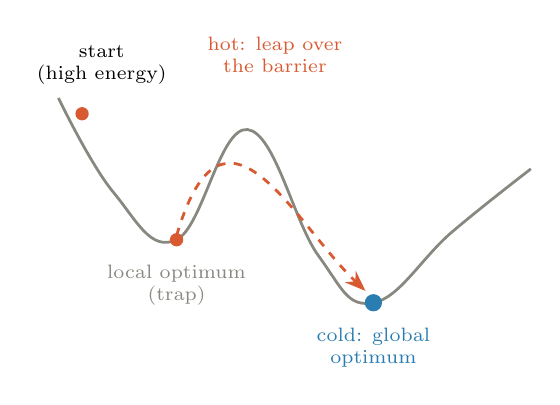
\begin{tikzpicture}[
          ball/.style={circle,fill=warm,inner sep=1.7pt},
          gball/.style={circle,fill=accent,inner sep=2.2pt}]
        \draw[muted,line width=1pt] plot[smooth,tension=0.7] coordinates
          {(0,3.0) (0.7,1.8) (1.5,1.2) (2.4,2.6) (3.3,1.0) (4.0,0.4) (5.0,1.3) (6,2.1)};
        \draw[warm,dashed,line width=1pt,-{Stealth}]
          (1.5,1.25) .. controls (2.1,3.3) and (3.0,1.4) .. (3.9,0.55);
        \node[ball]  at (0.3,2.8){};
        \node[ball]  at (1.5,1.2){};
        \node[gball] at (4.0,0.4){};
        \node[font=\scriptsize,align=center,anchor=south]             at (0.55,3.05){start\\(high energy)};
        \node[font=\scriptsize,align=center,text=warm,anchor=south]   at (2.75,3.2){hot: leap over\\the barrier};
        \node[font=\scriptsize,align=center,text=muted,anchor=north]  at (1.5,1.0){local optimum\\(trap)};
        \node[font=\scriptsize,align=center,text=accent,anchor=north] at (4.0,0.2){cold: global\\optimum};
      \end{tikzpicture}}
    \end{column}
    \begin{column}{0.36\textwidth}
      Under pure greedy descent the ball dies in the \textbf{local optimum}.
      \smallskip

      While \emph{hot}, SA tolerates the uphill leap over the barrier; while
      \emph{cold}, it settles and locks in.
      \smallskip

      Accepting $\Delta E>0$ with prob.\ $e^{-\Delta E/T}$ is exactly what
      escapes the trap.
    \end{column}
  \end{columns}
\end{frame}

\begin{frame}{Methods 2--4: LNS, Staged, ILS (\texttt{approach1})}
  \textbf{LNS (destroy \& repair).}
  \begin{itemize}
    \item \emph{Destroy:} BFS-grow a connected neighbourhood from a crossing-weighted seed vertex.
    \item \emph{Repair:} for each vertex, try $\sim$50 candidate positions, commit only the best
          strictly-improving one $\Rightarrow$ effectively greedy hill-climbing: fast descent, but stalls.
  \end{itemize}
  \medskip
  \textbf{Staged (\texttt{lns} $\to$ \texttt{sa}).} Greedy LNS burns down $\chi$ cheaply in the first
  30\% of the budget; SA then escapes the local optimum it left behind. Consistently among the best
  performers on dense graphs.
  \medskip

  \textbf{ILS.} Alternate full SA rounds with random \emph{kicks} (relocate $n/10$ random vertices),
  always restarting from the global best --- a different escape mechanism than temperature.
\end{frame}


\begin{frame}{LNS: Destroy \& Repair}
  \begin{itemize}
    \item \emph{Destroy:} BFS-grow a connected neighbourhood from a crossing-weighted seed vertex.
    \item \emph{Repair:} for each vertex, try $\sim$50 candidate positions, commit only the best
          strictly-improving one $\Rightarrow$ greedy hill-climbing: fast descent, but \textbf{stalls}.
  \end{itemize}
  \vfill
  \centering
  \resizebox{0.92\linewidth}{!}{%
  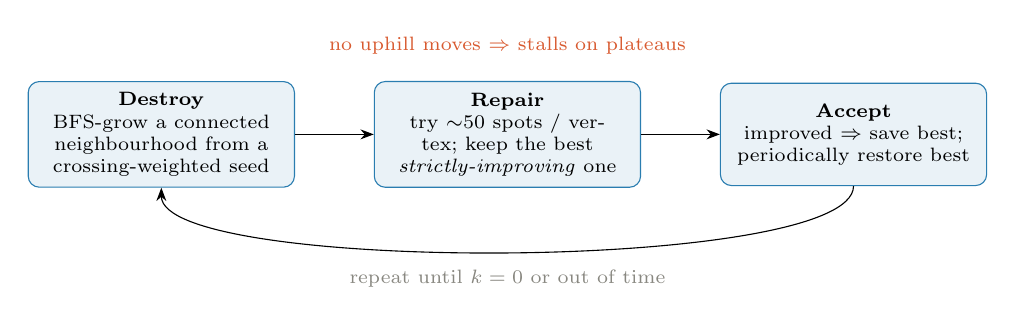
\begin{tikzpicture}[node distance=10mm,
      b/.style={rectangle,rounded corners,draw=accent,fill=accent!10,align=center,
                font=\scriptsize,inner sep=4pt,text width=3.1cm,minimum height=1.3cm}]
    \node[b](d){\textbf{Destroy}\\BFS-grow a connected neighbourhood from a crossing-weighted seed};
    \node[b,right=of d](r){\textbf{Repair}\\try $\sim$50 spots / vertex; keep the best \emph{strictly-improving} one};
    \node[b,right=of r](s){\textbf{Accept}\\improved $\Rightarrow$ save best; periodically restore best};
    \draw[-{Stealth}](d)--(r);
    \draw[-{Stealth}](r)--(s);
    \draw[-{Stealth}](s.south) .. controls +(0,-1.1) and +(0,-1.1) .. (d.south);
    \node[font=\scriptsize,text=warm]  at ($(r.north)+(0,0.45)$){no uphill moves $\Rightarrow$ stalls on plateaus};
    \node[font=\scriptsize,text=muted] at ($(r.south)+(0,-1.15)$){repeat until $k=0$ or out of time};
  \end{tikzpicture}}
\end{frame}

\begin{frame}{Staged \& ILS}
  \textbf{Staged} (\texttt{lns}$\to$\texttt{sa}): greedy LNS burns down $\chi$ in the first 30\% of the
  budget; SA then escapes the local optimum it left behind. \emph{Consistently among the best on dense graphs.}
  \vfill
  \begin{columns}[T]
    \begin{column}{0.66\textwidth}
      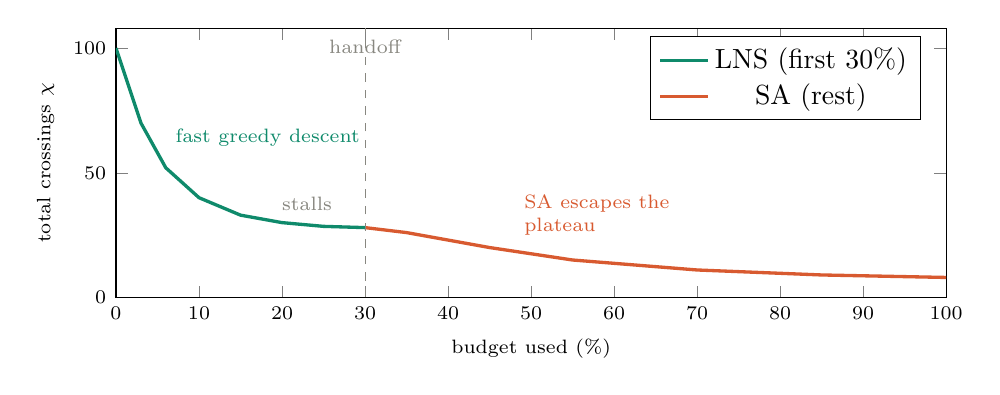
\begin{tikzpicture}
        \begin{axis}[width=\linewidth,height=5cm,
            xlabel={budget used (\%)},ylabel={total crossings $\chi$},
            xmin=0,xmax=100,ymin=0,ymax=108,legend pos=north east,
            tick label style={font=\scriptsize},label style={font=\scriptsize}]
          \addplot[teal,very thick] coordinates
            {(0,100)(3,70)(6,52)(10,40)(15,33)(20,30)(25,28.5)(30,28)};
          \addlegendentry{LNS (first 30\%)}
          \addplot[warm,very thick] coordinates
            {(30,28)(35,26)(45,20)(55,15)(70,11)(85,9)(100,8)};
          \addlegendentry{SA (rest)}
          \draw[muted,dashed] (axis cs:30,0)--(axis cs:30,108);
          \node[font=\scriptsize,text=teal,anchor=west]            at (axis cs:6,64){fast greedy descent};
          \node[font=\scriptsize,text=muted,anchor=south]          at (axis cs:23,31){stalls};
          \node[font=\scriptsize,text=warm,anchor=west,align=left] at (axis cs:48,33){SA escapes the\\plateau};
          \node[font=\scriptsize,text=muted,anchor=north]          at (axis cs:30,107){handoff};
        \end{axis}
      \end{tikzpicture}
    \end{column}
    \begin{column}{0.32\textwidth}
      \footnotesize
      \textbf{ILS:} alternate full SA rounds with random \emph{kicks} (relocate $n/10$ vertices),
      always restarting from the global best --- a different escape mechanism than temperature.
    \end{column}
  \end{columns}
\end{frame}
\section{Our Improvements}

\begin{frame}{Engineering: Spatial Grids Everywhere}
  \textbf{Problem:} naive checks are $O(m)$ or $O(n\cdot \deg)$ per move --- the move loop is the budget.
  \medskip
  \begin{itemize}
    \item \textbf{Edge grid} (bbox-based cell registration): crossing-delta of a move only tests
          edges in nearby cells --- no false negatives by construction.
    \item \textbf{Vertex grid}, kept in sync on every committed move: the validity check
          ``does any vertex lie on a moved edge?'' became $O(\text{local})$ instead of $O(n\cdot\deg)$.
          Verified exactly equivalent to the slow check; $\sim$10--25\% more moves/s.
    \item \textbf{Grid-accelerated initial repair}: resolves duplicate positions and
          vertex-on-edge overlaps of the input drawing (Automatic-8 previously produced
          \emph{invalid} output).
    \item \textbf{LNS budget discipline}: capped auto neighbourhood size and added an
          intra-iteration time check --- one LNS iteration can no longer overshoot the budget.
  \end{itemize}
\end{frame}

\begin{frame}{Phase 2: $k$-Critical Vertex Selection}
  \textbf{Observation:} phase 2 minimises the \emph{maximum}, but vertex selection was weighted by
  \emph{total} incident crossings --- poorly targeted at the bottleneck.
  \medskip

  \textbf{Improvement:} bias selection towards vertices incident to bottleneck edges
  (within band $\beta=2$ of the current $k$), with quadratic emphasis:
  \[
    w(v) = \sum_{\substack{e \ni v \\ \mathrm{cr}(e) \ge k-\beta}} \bigl(\mathrm{cr}(e)-(k-\beta)+1\bigr)^2
    \;+\; \text{base mass}
  \]
  \begin{itemize}
    \item Base mass is \emph{scaled to the critical mass} ($\sim$75\% of picks stay critical at any $n$);
          a fixed base constant would drown the signal on large graphs.
    \item Rebuilds of the selection table are rate-limited (full rebuild is $O(n+m)$).
  \end{itemize}
  \medskip
  \textbf{A/B (Automatic-7, 2\,min, same seeds):} $k = 55/61$ with $k$-critical selection
  vs.\ $77/75$ without.
\end{frame}

\begin{frame}{The Automatic-8 Story: Don't Trust the Input Drawing}
  \textbf{Symptom:} $k\approx 10\,000$ and $\sim$12\,min of setup before the solver even starts.
  \medskip

  \textbf{Root cause:} we always started from the \emph{given} drawing ---
  $\sim$45M crossings, avg.\ 4\,561 crossings/edge. Local moves can never untangle that,
  and building the crossing tables alone takes minutes. The graph itself is nearly planar
  ($n=10\,466$, $m=20\,288 < 2n$, max.\ degree 5).
  \medskip

  \textbf{Fix --- constructive initial layouts} (\texttt{--init auto}):
  \begin{enumerate}
    \item \textbf{BFS snake}: BFS order placed along a boustrophedon grid path with per-cell jitter
          $\Rightarrow$ graph-close vertices land geometrically close.
    \item \textbf{Barycenter smoothing} (50 rounds): pull each vertex to the mean of its neighbours,
          rescale the bounding box to the canvas each round (prevents collapse).
    \item \textbf{Auto-selection}: sample-estimate crossing density of
          \{input, snake, snake+smooth\}, keep the sparsest (protects curated inputs).
  \end{enumerate}
\end{frame}

\begin{frame}{Initial Layout: Measured Impact (Automatic-8)}
  \begin{center}
    \begin{tabular}{lrrr}
      \toprule
      & \textbf{input} & \textbf{BFS snake} & \textbf{+ smoothing} \\
      \midrule
      avg.\ crossings / edge & 4\,561 & 105 & \textbf{14} \\
      est.\ total crossings  & $\sim$45M & $\sim$0.9M & $\sim$0.15M \\
      \bottomrule
    \end{tabular}
  \end{center}
  \medskip
  \begin{itemize}
    \item Setup time: $\sim$12\,min $\to$ \textbf{$\sim$8\,s} (crossing tables shrink 250$\times$)
    \item 3-minute run: $k = 9\,958$ (old, 15\,min!) $\to$ 247 (snake) $\to$ \textbf{52} (snake + smoothing)
    \item Smoothed layout now wins the auto-selection on \emph{all nine} graphs
  \end{itemize}
\end{frame}

\begin{frame}{Stop Paying for Restarts: \texttt{restoreBest} Skip}
  \textbf{Measured:} on Automatic-8, phase 1 ran 95 temperature waves; each wave-end restart
  from the best solution recomputes \emph{all} crossings from scratch ---
  \textbf{32\,s of a 120\,s phase (27\% of the budget)}.
  \medskip

  \textbf{Fix:} skip the restore when the current state already matches the best
  ($k = k_{\text{best}}$ and $\chi$ within 1\% of $\chi_{\text{best}}$) --- which is the common case
  at the end of a low-temperature wave. Same rule added to the periodic LNS restart.
  \medskip

  \textbf{Effect (Automatic-8, phase 1, 120\,s):} $342$k $\to$ \textbf{1.01M moves} ($3\times$).
\end{frame}

\begin{frame}{Results: Before vs.\ After (same seeds, validated outputs)}
  \begin{center}
    \begin{tabular}{lrrrr}
      \toprule
      \textbf{Graph} & $n$ / $m$ & \textbf{Budget} & \textbf{Old pipeline} & \textbf{New pipeline} \\
      \midrule
      Automatic-1 & 50 / 202        & 1\,min  & 9 (5\,min)        & 9 \\
      Automatic-4 & 196 / 571       & 1\,min  & 7 (best ever, 5\,min) & \textbf{7} \\
      Automatic-6 & 200 / 3\,000    & 1\,min  & 633 (15\,min)     & 772 \\
      Automatic-7 & 500 / 1\,740    & 1\,min  & 45 (15\,min)      & 52 \\
      Automatic-8 & 10\,466 / 20\,288 & 3\,min & 9\,958 (15\,min) & \textbf{52} \\
      \bottomrule
    \end{tabular}
  \end{center}
  \medskip
  \begin{itemize}
    \item Small graphs reach their former best-ever values with a fraction of the budget.
    \item Automatic-8 improves by \textbf{two orders of magnitude} --- and the curve was still falling.
  \end{itemize}
\end{frame}

\begin{frame}{Lessons Learned \& Next Steps}
  \textbf{Lessons.}
  \begin{itemize}
    \item \textbf{Seed variance is huge}: identical code, 60\,s, seeds 42--45 on Automatic-4
          gave $k\in\{9,15,22,17\}$. A perceived ``regression'' was largely luck accumulated
          over many long runs. $\Rightarrow$ compare only with multiple identical seeds and equal budgets.
    \item \textbf{Measure before optimising}: the two biggest wins (initial layout, restart cost)
          came from profiling, not from tuning the annealing schedule.
    \item The \emph{starting point} matters more than the search on near-planar instances.
  \end{itemize}
  \medskip
  \textbf{Next steps.}
  \begin{itemize}
    \item Overnight long-budget runs on all nine graphs (in progress).
    \item Stronger initialisation (force-directed refinement) to push Automatic-8 towards
          the $k\approx 12$ reported by other teams.
    \item Phase-2 move throughput on the largest instances.
  \end{itemize}
\end{frame}

\end{document}
